\chapter{Model Predictive Control}

Model Predictive Control is a \textbf{\textit{feed back control}} algorithm that uses a model to make predictions about future outcomes of the process. Based on these predicted outcomes a control action can be implemented that optimizes the desired output. MPC can handle MIMO systems that is generally not possible using simple control algorithms such as PID. 

\begin{figure}[h!]
	\centering
	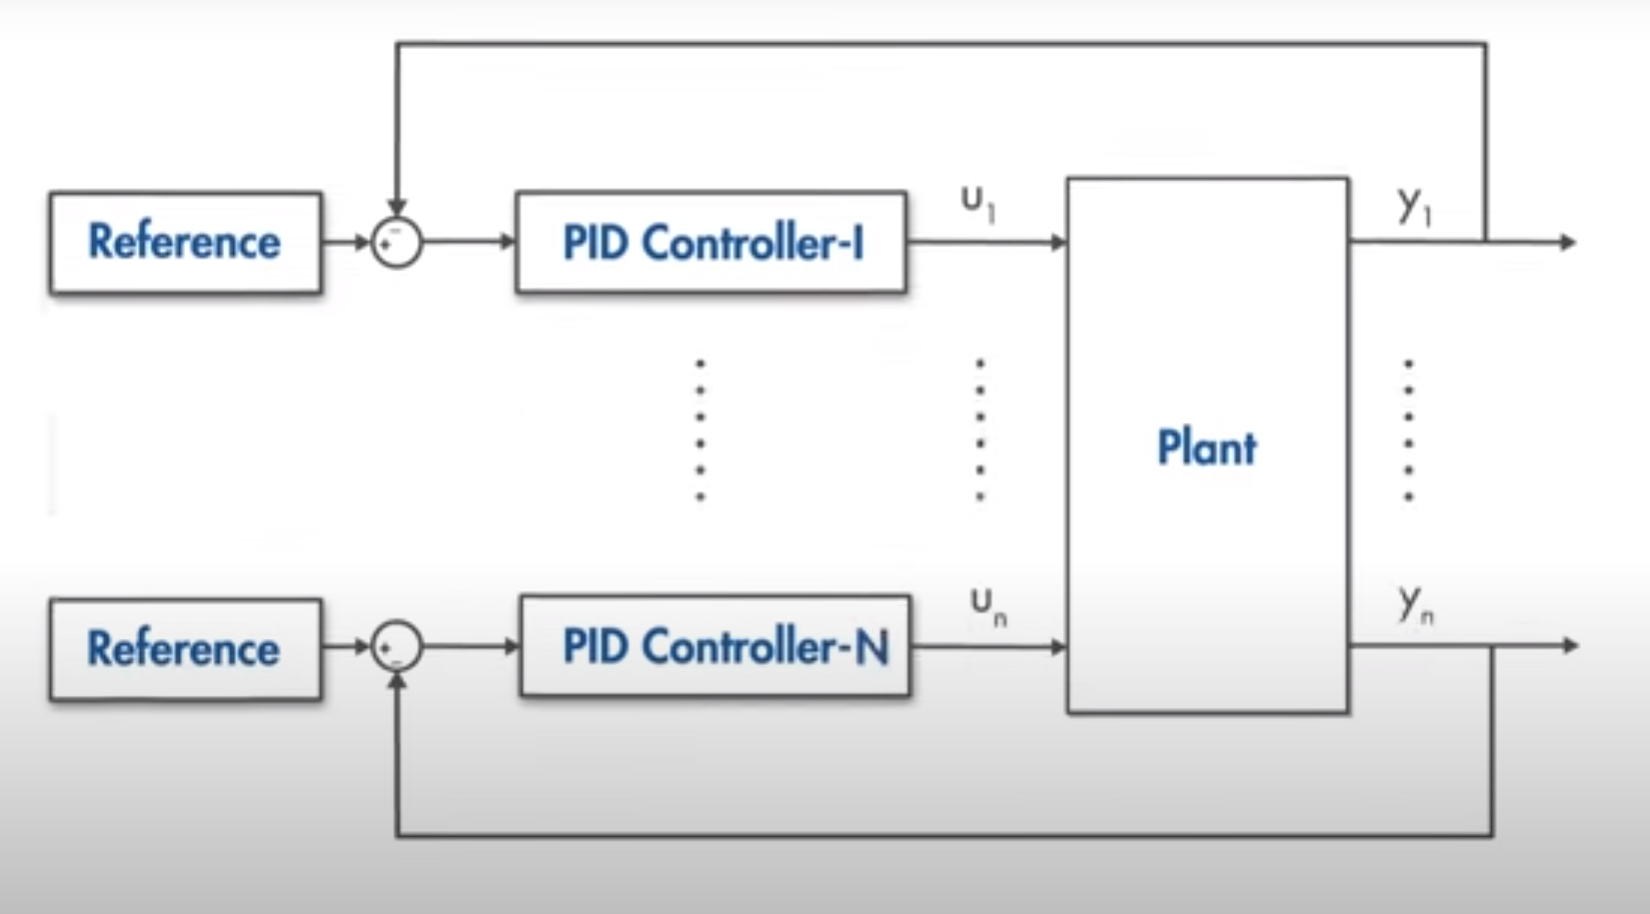
\includegraphics[width=\linewidth]{Bilder/Part2_MPC_MIMO_Application.PNG}
	\caption{MPC is a better option for MIMO systems}
\end{figure}

